\documentclass[english,14pt,a4paper]{article}
\usepackage[T1]{fontenc}
\usepackage{babel}
\usepackage{graphicx}
\usepackage{amsmath}
\usepackage{tikz}
\usepackage{amssymb}
\usepackage{qcircuit}
\usepackage{braket}
\usetikzlibrary{arrows.meta}
\usepackage{titlesec}

\title{How to create superposition of quantum states?}
\author{Vadym Shvydkyi}


\begin{document}
	\maketitle
	\tableofcontents
	\pagebreak
	\section{Introduction to quantum information science}
	\subsection{Qubit} \ \ \ \
	First of all, let us introduce such a concept as a \textit{qubit}. If in classical computer science we used either only \textit{0} or only \textit{1} to perform calculations, store and transmit information, in quantum computer science we can use superposition of 0 or 1. In Dirac notation we can describe a qubit as follows:
	\begin{equation}
		\ket{\psi}  = \alpha | 0 \rangle + \beta | 1 \rangle
	\end{equation}
	
	The numbers $\alpha$ and $\beta$ are coplex numbers that represent the probability of measuring state $| 0 \rangle $ or state $| 1 \rangle $. In turn, $| 0 \rangle $ and $| 1 \rangle $ form the computational basis of states, which is an orthonormal basis in the given vector space. 
	
	The numbers $\alpha$ and $\beta$ satisfy this equality $|\alpha|^2 + |\beta|^2 = 1$, so we can rewrite qbit in such form:
	\begin{equation}
		| \psi \rangle = e^{i\phi}( \cos(\frac{\eta}{2})| 0 \rangle + \sin(\frac{\eta}{2})e^{i\theta}| 1 \rangle)
	\end{equation} 
	 
	\begin{figure}[!htbp] %Bloch sphere
		\centering
		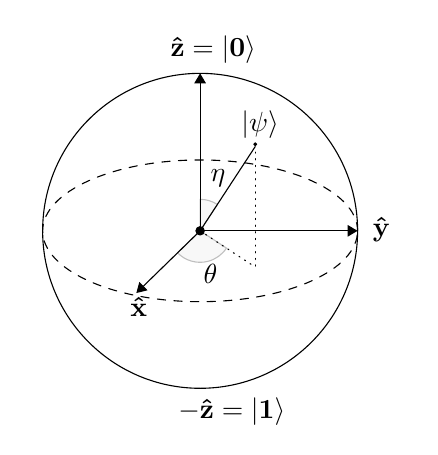
\begin{tikzpicture}[line cap=round, line join=round, >=Triangle]
			\clip(-2.19,-2.49) rectangle (2.66,2.58);
			\draw [shift={(0,0)}, lightgray, fill, fill opacity=0.1] (0,0) -- (56.7:0.4) arc (56.7:90.:0.4) -- cycle;
			\draw [shift={(0,0)}, lightgray, fill, fill opacity=0.1] (0,0) -- (-135.7:0.4) arc (-135.7:-33.2:0.4) -- cycle;
			\draw(0,0) circle (2cm);
			\draw [rotate around={0.:(0.,0.)},dash pattern=on 3pt off 3pt] (0,0) ellipse (2cm and 0.9cm);
			\draw (0,0)-- (0.70,1.07);
			\draw [->] (0,0) -- (0,2);
			\draw [->] (0,0) -- (-0.81,-0.79);
			\draw [->] (0,0) -- (2,0);
			\draw [dotted] (0.7,1)-- (0.7,-0.46);
			\draw [dotted] (0,0)-- (0.7,-0.46);
			\draw (-0.08,-0.3) node[anchor=north west] {$\theta$};
			\draw (0.01,0.9) node[anchor=north west] {$\eta $};
			\draw (-1.01,-0.72) node[anchor=north west] {$\mathbf {\hat{x}}$};
			\draw (2.07,0.3) node[anchor=north west] {$\mathbf {\hat{y}}$};
			\draw (-0.5,2.6) node[anchor=north west] {$\mathbf {\hat{z}=|0\rangle}$};
			\draw (-0.4,-2) node[anchor=north west] {$-\mathbf {\hat{z}=|1\rangle}$};
			\draw (0.4,1.65) node[anchor=north west] {$|\psi\rangle$};
			\scriptsize
			\draw [fill] (0,0) circle (1.5pt);
			\draw [fill] (0.7,1.1) circle (0.5pt);
		\end{tikzpicture}
		\caption{Bloch sphere for $| \psi \rangle $}
		\label{fig:blochsphere1}
	\end{figure} 
	We can disregard the factor $e^{i\phi}$ since we have no way to measure it. So finally we can characterize the qubit as follows:
	\begin{equation}
		\ket{\psi} = \cos(\frac{\eta}{2})| 0 \rangle + \sin(\frac{\eta}{2})e^{i\theta}| 1 \rangle
	\end{equation}  
	This form can be shown as a unit vector on the sphere. This sphere, called the Bloch sphere. Since $\ket{0}$ and $\ket{1}$ are a basis, we can characterize the state vector as a vector, namely
	\[
		\ket{\psi} = \alpha \ket{0} + \beta\ket{1} \equiv 
		\begin{pmatrix} \alpha \\ \beta \\ \end{pmatrix}  
	\]
	
	If we have two qubits, each of which has its own computational basis, then the qubit that characterizes the whole system belongs to the vector space that was obtained as a result of the Cartesian product of the first two vector spaces, and the basis of the new vector space forms a new computational basis for the whole system. Or in the formalism of quantum mechanics if we have \textit{n} qubits, the whole system is describe be the cubit $\ket{\psi_{1 \ldots n}}$:
	
	\begin{equation}
		\ket{\psi_{1 \ldots n}} = \ket{\psi_1} \otimes \ket{\psi_2} \otimes \ldots \otimes \ket{\psi_n} 
	\end{equation}
	
	\subsection{Quantum Circuits and Quantum Gates}
	
	 \ \ \ \ The device, which we can call a quantum computer we can describe as a \textit{quantum circuit}, which consists of \textit{registers} and \textit{quantum gates}. In the figure we can see an example of a quantum circuit for Deutsch's algorithm. Quantum gates by analogy with classical computers can be represented as logic elements that act on a qubit and as a result of measurements we perform calculations on a quantum computer.
	 
	\begin{figure}[!htbp] %Deutsch
		\[
		\Qcircuit @C=1em @R=.7em {
			\lstick{\ket{0}} & \gate{H} & \multigate{1}{U_f} & \gate{H} & \qw \\
			\lstick{\ket{1}} & \gate{H} & \ghost{U_f} & \qw & \qw \\
		}
		\]
		\caption{Deutsch's algorithm}
		\label{deutsch}
	\end{figure}
	 
	
	According to the postulate of quantum theory that the evolution of a quantum system in time is described by a \textit{unitary operator}, so the matrix which represents this operator must be unitary. Consider in detail these matrices. We know that these are 2x2 matrices that are unitary. More generally, if a quantum gate acts on multiple registers, i.e. on multiple qubits, then it is a matrix $2^n\text{x}2^n$, which belongs to the $\text{SU}(2^n)$. The qubit we obtained after the quantum gate action is expressed as the multiplication of the operator by the qubit, $\ket{\psi'} = U \ket{\psi}$. \\
	
	Here are a few systems that can be described as qubits: 
	\begin{table}[h]
	\centering
	\begin{tabular}{|c|c|} 
		\hline
		Degree of freedom & Possible basis states $\ket{0}$, $\ket{1} $\\ 
		\hline
		Spin $\frac12$  & $\ket{m = \frac12}$, $\ket{m = - \frac12}	$  \\ 

		Photon polarization & $\ket{\text{horizontal}}$, $\ket{\text{vertical}}$ \\

		Two-level atom & $\ket{\text{groundstate}}$, $\ket{\text{exitedstate}}$ \\ 
		\hline
	\end{tabular}
	\end{table}
	
	\subsection{Examples of quantum gates} \ \ \ \ 
	Here we would like to provide examples of quantum gates that we will use in the future. Some of them were obtained directly and from the rotation matrices or derived from the truth table for each case. 
	
	\subsubsection{X, Y, Z gates}\ \ \ \
	\(X  \ Y \ Z\) quantum gates represent a rotation about the $\hat{x}, \ \hat{y}, \ \hat{z}$ axis respectively on the Bloch sphere. The matrices of these operators are Pauli matrices for each of the axes. 
	
	\subsubsection{Hadamard gate}\ \ \ \
	The Hadamard operator will be discussed more depth in later chapters, as it is used to create a superposition of the simplest states 0 and 1 behind such a rule. 
	
	\[
		H \ket{0} = \frac{\ket{0} + \ket{1}}{\sqrt{2}} \equiv \ket{+}, \ H \ket{1} = \frac{\ket{0} - \ket{1}}{\sqrt{2}} \equiv \ket{-}
	\]
	\begin{equation}
	H = \frac{1}{\sqrt{2}} \begin{pmatrix} 1 & 1 \\ 1 & -1 \end{pmatrix}
	\end{equation}
	
	\subsubsection{CNOT gate}\ \ \ \
	This operator is the analog of CNOT in classical computers. It can be described by the following rule: $\ket{xy} = \ket{x x \oplus y}; x, y \in \mathbb{Z}_2$, where the $x$ is \textit{control qubit} and $y$ is \textit{target qubit}. Let $D$ be an operator for a CNOT gate then we can describe it in this way $D = \ket{0}\bra{0} \otimes \mathbb{I} + \ket{1}\bra{1} \otimes X$. Here $X$ operator plays the role of logical element \textit{Not}. In this way we can create a generic controlled operator \textit{C-A} which applied on target qubit in such way: $\ket{0}\bra{0} \otimes \mathbb{I} + \ket{1}\bra{1} \otimes A $
	\subsubsection{Rotation Operators about the Bloch basis}\ \ \ \
	Since the Lie algebra of the group $\text{SU}(2)$ is isomorphic to the Lie algebra of the group $\text{SO}(3)$, it is a very useful fact that operators can be represented as rotations of the Bloch sphere. For each axis we have an operator represented in this form:
	\[
		R_{\hat{x}}(\eta) = e^{-\frac{i\eta}{2}X} = \begin{pmatrix}
			\cos(\frac{\eta}{2}) & -i\sin(\frac{\eta}{2}) \\
			-i\sin(\frac{\eta}{2}) & \cos(\frac{\eta}{2}) \\
		\end{pmatrix}	
	\]
	\[
	R_{\hat{y}}(\eta) = e^{-\frac{i\eta}{2}Y} = \begin{pmatrix}
		\cos(\frac{\eta}{2}) & -\sin(\frac{\eta}{2}) \\
		\sin(\frac{\eta}{2}) & \cos(\frac{\eta}{2}) \\
	\end{pmatrix}	
	\]
	\[
	R_{\hat{z}}(\eta) = e^{-\frac{i\eta}{2}Z} = \begin{pmatrix}
		e^{-i\frac{\eta}{2}} & 0 \\
		0 &  e^{i\frac{\eta}{2}}\\
	\end{pmatrix}	
	\]
	
	That is, in general we can represent a unitary operator as a rotation operator in three-dimensional space by $\eta$ around an axis in the direction of the unit vector $\hat{n}$.
	 \begin{equation}
	 R_{\hat{n}}(\eta) = e^{-\frac{i}{2}\eta \hat{n}\cdot \vec{\sigma}}
	\end{equation}
	\subsection{Bures Fidelity} \ \ \ \
	\textit{Bures fidelity} offers a precise assessment of the distinguishability between two density matrices. In this section, we will employ Bures fidelity to validate the findings from the preceding section. The fidelity is defined as: 
	\begin{equation}
		F(\rho_1, \rho_2) = tr(\rho_1^{1/2}\rho_2\rho_1^{1/2})
	\end{equation}
	
	The value of F lies between $0$ and $1$, where $F = 1$ denotes that the states are identical. For the pure state $\rho_1 = \ket{\psi}\bra{\psi}$ we can define the fidelity \[F = \bra{\psi}\rho_2 \ket{\psi}\].
	
	
	\pagebreak
	\section{Creation of a superposition} 
	\subsection{Problem formulation} \ \ \ \
	Consider such a problem that we need to create a superposition from the general state of $|\psi\rangle$, which in generality looks like $ \frac{|\psi\rangle + |\psi^{\perp}\rangle}{\sqrt{2}}$. For this purpose, take a look at the given device, which we can represent as operator $\hat{G}$:
	\begin{equation}\label{popa_muravia}
		|\psi \rangle_a | Q \rangle _b \longmapsto \frac{|\psi \rangle_a + |\psi^{\perp} \rangle_a}{\sqrt{2}} |Q_{\psi} \rangle_b
	\end{equation} 
	
	Consider the registers of this device: in register $a$ we have an initial cubit whose superposition we want to create, register $b$ is the prepared cubit that we use to create the superposition in register $a$. At the output we get in register $a$ the superposition of the general $|\psi \rangle$ state and also the $|Q _{\psi} \rangle$. \\ 
	
	Since we can rewrite the $|\psi \rangle$ state as a superposition of the basis states, we can consider this equation in such form:
	
		$\hat{G}|\psi \rangle_a | Q \rangle _b = \hat{G}(\alpha |0 \rangle_a  + \beta |1 \rangle_a)| Q \rangle _b = \alpha \hat{G}|0 \rangle_a | Q \rangle _b + \beta \hat{G}|1 \rangle_a | Q \rangle _b = \\ = \alpha \hat{G}|1 \rangle_a | Q_0 \rangle _b + \beta \hat{G}|0 \rangle_a | Q_1 \rangle _b$. \\
		
	In these calculations we no longer see that this operator does not fulfill one of the points of the definition of an unitary operator, namely its linearity. And since the operator cannot be an unitary operator, this gate element can not be realized. \\
	
	So we propose to consider a problem in which our goal is to create a state that is as close as possible to the state we are interested in. To calculate the closeness of the states we will use Bures distance. 
	\subsection{Respectively Position of a States on the Bloch Sphere}\ \ \ \
	As already described in Chapter 1.3.4 we can consider unitary operators as rotations of a unit vector on the Bloch sphere. This is why I think it is very relevant to study how one can represent the states of qubits on the flea sphere. \\
	
	Initially, we can denote the unit vector $\hat{n} = \cos(\theta)\sin(\eta) \hat{x} + \sin(\theta)\sin(\eta)\hat{y} + +\cos(\eta)\hat{z}$. This unit vector $\hat{n}$ represents the state $\ket{\psi} = \cos(\frac{\eta }{2})\ket{0} + \sin(\frac{\eta}{2}) e^{i\theta}\ket{1}$, the state $\ket{\psi^{\perp}}$ which s perpendicular to the state $\ket{\psi}$ is $\ket{\psi^{\perp}} = -\sin{\frac{\eta}{2}}e^{-i\theta} \ket{0} ++ \cos(\frac{\eta}{2})\ket{1}$, which suggests that the angles have been altered in this way: $ \eta \rightarrow \eta + \pi $ and $ \theta \rightarrow \theta$. So it is ease to see that vector $-\hat{n}$ is orthogonal to $\hat{n}$. Therefore, the 6 main directions $\pm \hat{x}, \ \pm \hat{y}, \ \pm \hat{z}$ can form the basis. If $\hat{z} \equiv \ket{0} \text{and} \ -\hat{z} \equiv \ket{1}$, $\pm \hat{x} \equiv \frac{\ket{0} \pm \ket{1}}{\sqrt{2}}$ which is also called $\ket{\pm}$. In addition, I think it should be clarified that these pairs of vectors are eigenvectors of the pauli matrices of the corresponding axes. 
	\[
	\sigma_x = \ket{0}\bra{1} + \ket{1}\bra{0}
	\]
	\[
	\sigma_y = -i\ket{0}\bra{1} + \ket{1}\bra{0}
	\]
	\[
	\sigma_z = \ket{0}\ket{0} - \ket{1}\bra{1}
	\]
	
	Since we already know that for the $\ket{\psi}$ cubit we can set the $\vec{\psi}$ vector on the Bloch sphere, then the vector $-\vec{\psi}$ represents $\ket{\psi^{\perp}}$ on a Bloch sphere. Based on this information we can describe our target state $\ket{\Psi} = \frac{\ket{\psi} + \ket{\psi^{\perp}}}{\sqrt{2}}$ as a vector $\vec{\Psi}$ that will be between $\vec{\psi}$ and $-\vec{\psi}$, as is shown on the picture. 
	\begin{figure}[!htbp] %Bloch sphere
		\centering
		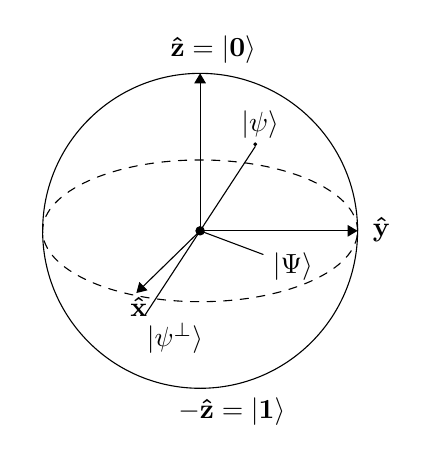
\begin{tikzpicture}[line cap=round, line join=round, >=Triangle]
			\clip(-2.19,-2.49) rectangle (2.66,2.58);
			
			\draw(0,0) circle (2cm);
			\draw [rotate around={0.:(0.,0.)},dash pattern=on 3pt off 3pt] (0,0) ellipse (2cm and 0.9cm);
			\draw (0,0)-- (0.70,1.07);
			\draw (0,0)-- (-0.70,-1.07);
			\draw (0, 0) -- (0.80, -0.30);
			\draw (0.8,-0.15) node[anchor=north west] {$\ket{\Psi}$};
			\draw [->] (0,0) -- (0,2);
			\draw [->] (0,0) -- (-0.81,-0.79);
			\draw [->] (0,0) -- (2,0);
			\draw (-1.01,-0.72) node[anchor=north west] {$\mathbf {\hat{x}}$};
			\draw (2.07,0.3) node[anchor=north west] {$\mathbf {\hat{y}}$};
			\draw (-0.5,2.6) node[anchor=north west] {$\mathbf {\hat{z}=|0\rangle}$};
			\draw (-0.4,-2) node[anchor=north west] {$-\mathbf {\hat{z}=|1\rangle}$};
			\draw (0.4,1.65) node[anchor=north west] {$|\psi\rangle$};
			\draw (-0.8,-1.05) node[anchor=north west] {$\ket{\psi^{\perp}}$};
			\scriptsize
			\draw [fill] (0,0) circle (1.5pt);
			\draw [fill] (0.7,1.1) circle (0.5pt);
		\end{tikzpicture}
		\caption{Bloch sphere for $\ket{\Psi} $}
		\label{fig:blochsphere2}
	\end{figure} 
	Let us consider in detail the superposition on the example of simple states, i.e. $\ket{0}$ and $\ket{1}$. 
	
	
\end{document}